\adparagraph{Spearman Distance}
In Figure \ref{fig:footruledistance} are the results of the Footrule distance tests. As for Kendall distance it is normalized to be between 0 and 1 where if 0 the list are equal. 

In general the tendencies are very similar to those of Kendall distance the approaches follow the same curve with all most the same distance jumps between the group sizes. 

Not surprisingly SF performs the best in this test. This is due to it have a natural advantage when using Footrule distance as they are based on the same principle. This somewhat deems its result in this test invalid. 

Average again perform the worst when looking at the Footrule distance results. This is for the same reason as with the Footrule test, Average does not take the rank of items into account.

For MC and BC we get some interesting results. They still follow each other really close. However in this test BC performs best on the small groups and is later out scaled by MC but first when the group sizes reaches approximately 30 members.

\begin{figure}[H]
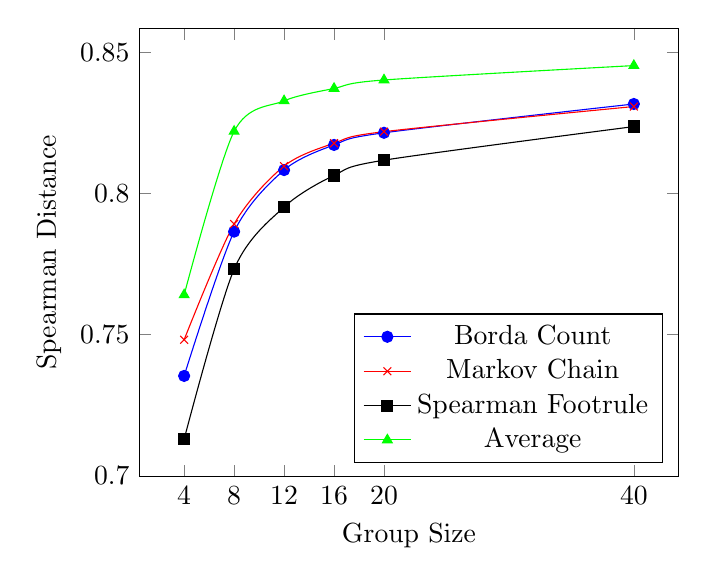
\begin{tikzpicture}
    \begin{axis}[
        xlabel=Group Size,
        ylabel=Spearman Distance,
        xtick = {4,8,12,16,20,40},
        legend pos=south east]
    \addplot[smooth,mark=*,blue] plot coordinates {
        (4,0.7354)
        (8,0.7865)
        (12,0.8083)
        (16,0.8172)
        (20,0.8215)
        (40,0.8317)
    };
    \addlegendentry{Borda Count}

    \addplot[smooth,color=red,mark=x] plot coordinates {
            (4,0.7482)
            (8,0.7892)
            (12,0.8097)
            (16,0.8178)
            (20,0.8219)
            (40,0.8308)
        };
    \addlegendentry{Markov Chain}
    
        \addplot[smooth,color=black,mark=square*] plot coordinates {
            (4,0.7130)
            (8,0.7732)
            (12,0.7952)
            (16,0.8064)
            (20,0.8118)
            (40,0.8237)
        };
    \addlegendentry{Spearman Footrule}
    
    \addplot[smooth,color=green,mark=triangle*] plot coordinates {
            (4,0.7641)
            (8,0.822)
            (12,0.8328)
            (16,0.8372)
            (20,0.8402)
            (40,0.8453)
        };
    \addlegendentry{Average}
    
    \end{axis}
\end{tikzpicture}
\caption{Results using Footrule distance} \label{fig:footruledistance}
\end{figure}
